\documentclass[11pt]{article}
\usepackage[utf8]{inputenc}
\usepackage{fancyhdr}
\usepackage[english]{babel}
\usepackage{graphicx}
\usepackage{array}
\usepackage{amsmath}
\usepackage{amssymb}
\usepackage{mathtools}
\usepackage{algorithmicx}
\usepackage{algpseudocode}
\renewcommand{\baselinestretch}{1.0}
\usepackage[letterpaper, margin=0.75in]{geometry}
\DeclarePairedDelimiter{\ceil}{\lceil}{\rceil}
\pagestyle{fancy}
\lhead{}
\rhead{Yu Mi, yxm319. Algorithm HW2}
\begin{document}
	\title{Homework2 for EECS 340}
	\author{Yu Mi,yxm319}
	\maketitle
\section{Give a recursive algorithm to find the average (mean) value of an array of $2^k$ decimal numbers, where $k\in \mathbb{N}$.}
	\emph{Answer:} The proposed algorithm is as follow:
	
	\begin{algorithmic}
	\State \textbf{Algorithm A1}: Average($L$)
	\State \textbf{Data}: A list of $2^k$ decimal numbers $L$.
	\State \textbf{Result}: The average of all the numbers in $L$.
	\If {$L$.length()$=0$} 
		\State \Return $L[0]$
	\Else
		\State $length\gets L.length()$
		\State \Return $0.5\times$$($Average($L[0,length/2-1]+$Average($L[length/2,length]$)$)$
	\EndIf
	\end{algorithmic}
\section{R-12.6}
	\emph{Question}:Suppose we are given a set of telescope observation requests, specified by triples, of $(s_i, f_i, b_i)$, defining the start times, finish times, and benefits of each observation request as
	\begin{equation*}
		L={(1,2,5),(1,3,4),(2,4,7), (3,5,2), (1,6,3), (4,7,5), (6,8,7), (7,9,4)}
	\end{equation*}
	Solve the telescope scheduling problem for this set of observation requests.
	
\noindent	\emph{Answer}: The time of scheduling can be shown in Fig.\ref{fig:fig1}, the number in the bar means the value of such task. 
	\begin{figure}[h]
		\centering
		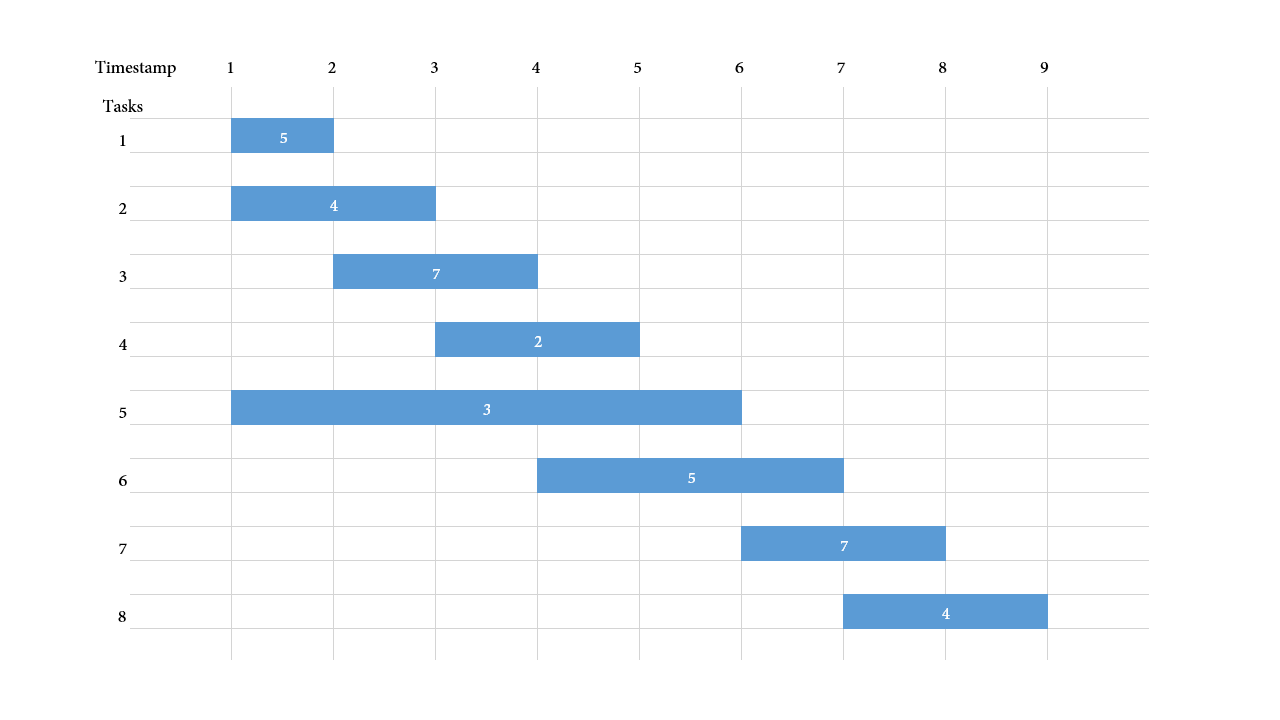
\includegraphics[width=0.62\textwidth]{Figure/FG1.png}
		\caption{Time of tasks}
		\label{fig:fig1}
	\end{figure}
	
	Based on what we have discussed on class, we can have a table of $B_i$ which stands for the maximum benefit that can be achieved with the first $i$ requests in the task list. 
	
	To fill this table, we follow the algorithm as follow:
	\begin{algorithmic}
	\State $B[0]\gets0$
	\For {$i$ = 1 to $n$ }
	\State     $B[i]\gets max(B[i-1],B[P[i]]+b_i)$
	\EndFor
	\end{algorithmic}
	
	Here the $P[i]$ stands for the array which gives the predecessor index for each request $i$, and $b_i$ means the value of each single task. The table is shown as Table \ref{tab:tab1}.
	\begin{table}[!hbp]
		\centering
		\caption{$B_i$ values}
			\begin{tabular}{c|c|c|c|c|c|c|c|c|c}
			\hline 
			\hline
			$i$  &$0 $& $1$ & $2$& $3$& $4$& $5$& $6$& $7$& $8$\\
			\hline
			$B_i$& 0  & 5   & 4  & 12 & 6  & 3  & 17 & 13 &21\\
			\hline
			\hline
			\end{tabular}
		\label{tab:tab1}
	\end{table}
	
	As we can see, the highest value is $B_8$, which includes task $1,3,6,8$ that we should select. The corresponding triples are $(1,2,5), (2,4,7),(4,7,5),(7,9,4)$.
\section{Implement \emph{det-bogoSort} in pseudocode using recursion}
	\emph{Answer}: This algorithm is described as follows:
	\begin{algorithmic}
	\State \textbf{Algorithm} BogoSort($S,L,L_{temp}$)
	\State \textbf{Data}: Input list $L$, as is described in the question, an initially empty set of lists $S$, and an initially empty list $L_{temp}$
	\State \textbf{Result}: A sorted copy of $L$
	\If {$size(L)=0$}
		\State $flag \gets true$
		\For {$i \gets 1 $ to $size(L_{temp})-1$}
			\If {$L_{temp}[i-1]>L_{temp}[i]$}
				\State $flag \gets false$
				\State \textbf{break}
			\EndIf
		\EndFor
		\If {$flag = true$}
			\State \Return $L_{temp}$
		\EndIf
	\Else
		\For {$i \gets 0$ to $size(L)-1$}
			\State $L_{temp}$.append($L[i]$)
			\State $L$.remove($i$)
			\State BogoSort($S,L,L_{temp}$)
		\EndFor
	\EndIf
	\end{algorithmic}
	
	NOTE: in the operations of lists, $L_{temp}$.append($L[i]$) means to append the element $L[i]$ at the end of list $L_{temp}$. And $L$.remove($i$) means to remove the $i$th element in list $L$.
\section{Write pseudo-code for a new recursive function \emph{moving-average}}
	\emph{Answer}: The algorithm is shown as follows:
	\begin{algorithmic}
	\State \textbf{Algorithm} moving-average($S,t_{start},t_{end}$)
	\State \textbf{Data}: Stock-price time series data $S$,a start time $t_{start}$, and a ending time $t_{end}$.
	\State \textbf{Result}: The average stock price from $t_{start}$ through $t_{end}$.
	\State $i\gets0$
	\If {$t_{start} = t_{end}$}
		\State \Return 0
	\EndIf
	\For {$i\gets t_{end}$ to $t_{start}$}
		\If {$t_{start}\%(i-t_{start})=0$ \textbf{and} ($(i-t_{start})$ is a power of 2)}
			\State \Return $\frac{i-t_{start}}{t_{end}-t_{start}}\times$ pow-of-two-average($S,t_{start},i$)+$\frac{t_{end}-i}{t_{end}-t{start}}\times$ moving-average($S,i,t_{end}$)
			\State \textbf{break}
		\EndIf
	\EndFor
	\State \Return 0
	\end{algorithmic}
\section{Write pseudo-code for a recursive function to compute \emph{checker-sum(A)$_{i,j}$} given the triple ($A,i,j$)}
	\emph{Answer}: The algorithm is shown as follows:
	\begin{algorithmic}
	\State \textbf{Algorithm} checker-sum($A,i,j$)
	\State \textbf{Data}: A matrix $A$, and index $i$ and $j$
	\State \textbf{Result}: The checkerboard sum of matrix $A$
	\If {$j>1$}
		\State \Return compute-row($A,i,j$) $-$ checker-sum($A,i,j-1$)
	\Else
		\State \Return compute-row($A,i,j$)
	\EndIf
	\end{algorithmic}

	\begin{algorithmic}
	\State \textbf{Algorithm} compute-row($A,i,j$)
	\State \textbf{Data}: A matrix $A$, and index $i$ and $j$
	\State \textbf{Result}: The checkerboard sum of row $j$ in matrix $A$
	\If {$i>1$}
		\State \Return $A(i,j)$ $-$ compute-row($A,i-1,j$)
	\Else
		\State \Return $A(i,j)$
	\EndIf
	\end{algorithmic}
\section{Read section 17.1 in the textbook and then solve the following problems}
\subsection{R-17.7}
	\emph{Question}: Show that the CLINQUE problem is in \emph{NP}
	
\subsection{C-17.3}
	\emph{Question}: Show that we can deterministically simulate in polynomial time any nondeterministic algorithm $A$ that runs in polynomial time and makes at most $O(\log n)$ calls to the \textbf{choose} method, where $n$ is the size of the input to $A$.
\end{document}